% Chapter 4
\chapter{Results \& Discussion} % Main chapter title
\label{Chapter4} % For referencing the chapter elsewhere, use \ref{Chapter4}
The CA model created in the previous chapter ran for 50 generations or time steps. An image was generated of the simulated Building Based Land Usage growth and it was saved. Additionally, the accuracy of the simulated growth was calculated and saved for each time step. A model without any validation and accuracy testing is ineffectual. For this reason a metric has to be employed to test the accuracy. The metric involved for this process is the Kappa coefficient (also known as Cohen's Kappa coefficient). This metric returns a score that expresses the level of agreement between two annotators and estimate the ground truth. It is utilised vastly in Machine Learning problems, but has also seen its usage in CA urban modelling\cite{m1,m2,m3,m4,m5,m6,m7,m8,m9}. The formula to calculate this coefficient is as follows:\cite{sklearn}
\begin{center}
$\kappa = (p_o - p_e) / (1 - p_e)$
\end{center}
The variable $p_o$ is the the observed agreement ratio (observed accuracy), and the variable $p_e$ is the expected agreement (expected accuracy).

The Table \ref{table:kap} below shows values and their respective magnitudes guidelines for the Kappa coefficient\cite{kappatb}.
\begin{table}[H]
\centering
\caption{Interpreting the Kappa coefficient magnitude}
\label{table:kap}
\begin{tabular}{@{}ll@{}}
\toprule
\multicolumn{1}{l}{Values} & \multicolumn{1}{l}{Magnitude guideline} \\ \midrule
$\kappa \leq 0$                & No agreement                            \\
$0 \leq \kappa \leq 0.20$                     & Slight agreement                        \\
$0.21 \leq \kappa \leq 0.40$                  & Fair agreement                          \\
$0.41 \leq \kappa \leq 0.60$                  & Moderate agreement                      \\
$0.61 \leq \kappa \leq 0.804$                  & Substantial agreement                   \\
$0.81 \leq \kappa \leq 1$                     & Almost perfect agreement                \\ \bottomrule
\end{tabular}
\end{table}
Besides the Kappa coefficient the following additional metrics have been used in similar CA urban modelling research:
\begin{itemize}
\item Visual comparisons between of modelled and real growth\cite{om1,om6,m8}
\item Ratio between modelled urban px and number of real urban px\cite{om2,om5}
\item Regression analysis (r-square values)\cite{om3}
\item The Lee–Sallee index\cite{om4,m1}
\item The Moran's I index\cite{om6}
\item Other spatial indices
\end{itemize}

Besides the Kappa coefficient the the Visual Comparison metric was chosen as an additional metric to validate the accuracy of the final CA model. For this approach two separate techniques were utilised. The first involved creating a GIF image from all the images that were saved during the duration of the CA model execution. The GIF was created using imgflip\footnote{\url{https://imgflip.com/gif-maker}}. The GIF can be found at this research study's repository.\footnote{\url{https://github.com/AM-ops/Hons-Project-Documentation/blob/main/Hons-Project-Documentation-Final/Figures/gifs/Growth.gif}} A few snippets from the GIF image are displayed below in Figure \ref{fig:gen50}.
\begin{figure}[H]
\begin{subfigure}{.5\textwidth}
  \centering
  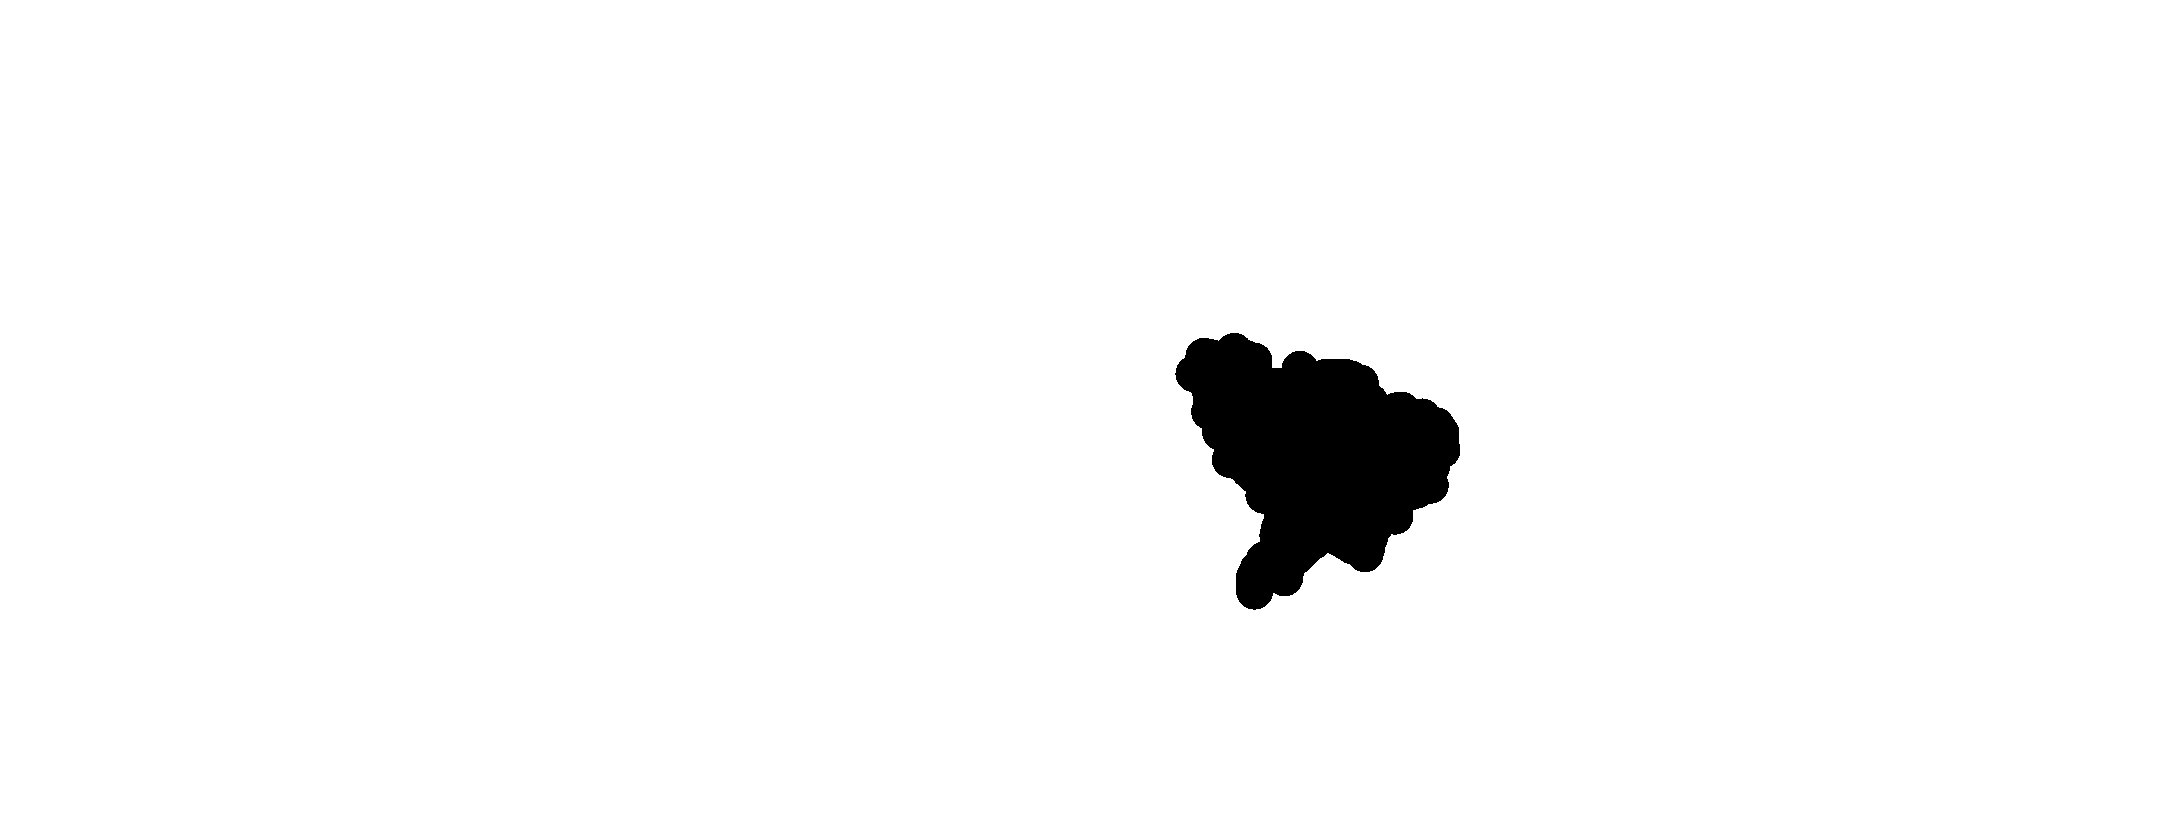
\includegraphics[width=1\linewidth]{Figures/Chapter4/generation-0-melusi}
  \caption*{Initial State}
\end{subfigure}
\begin{subfigure}{.5\textwidth}
  \centering
  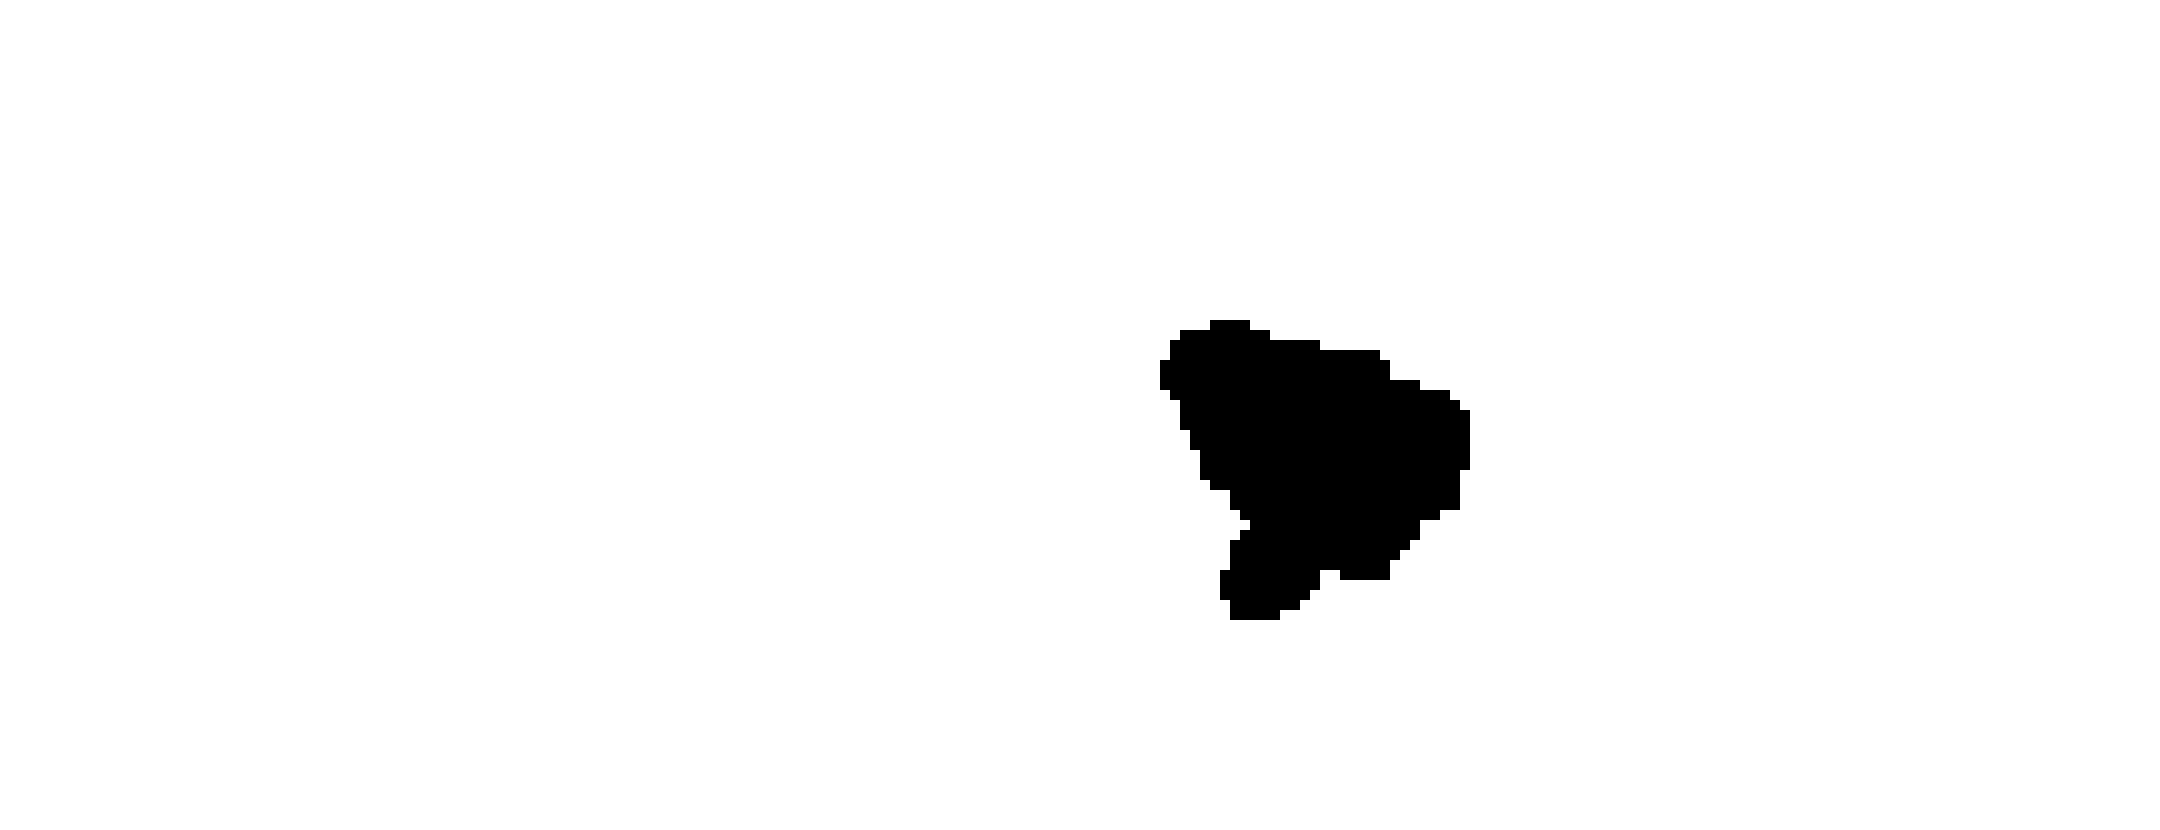
\includegraphics[width=1\linewidth]{Figures/Chapter4/generation-1-melusi}
  \caption*{Time step $t = 1$}
\end{subfigure}
\end{figure}

\begin{figure}[H]
\begin{subfigure}{.5\textwidth}
  \centering
  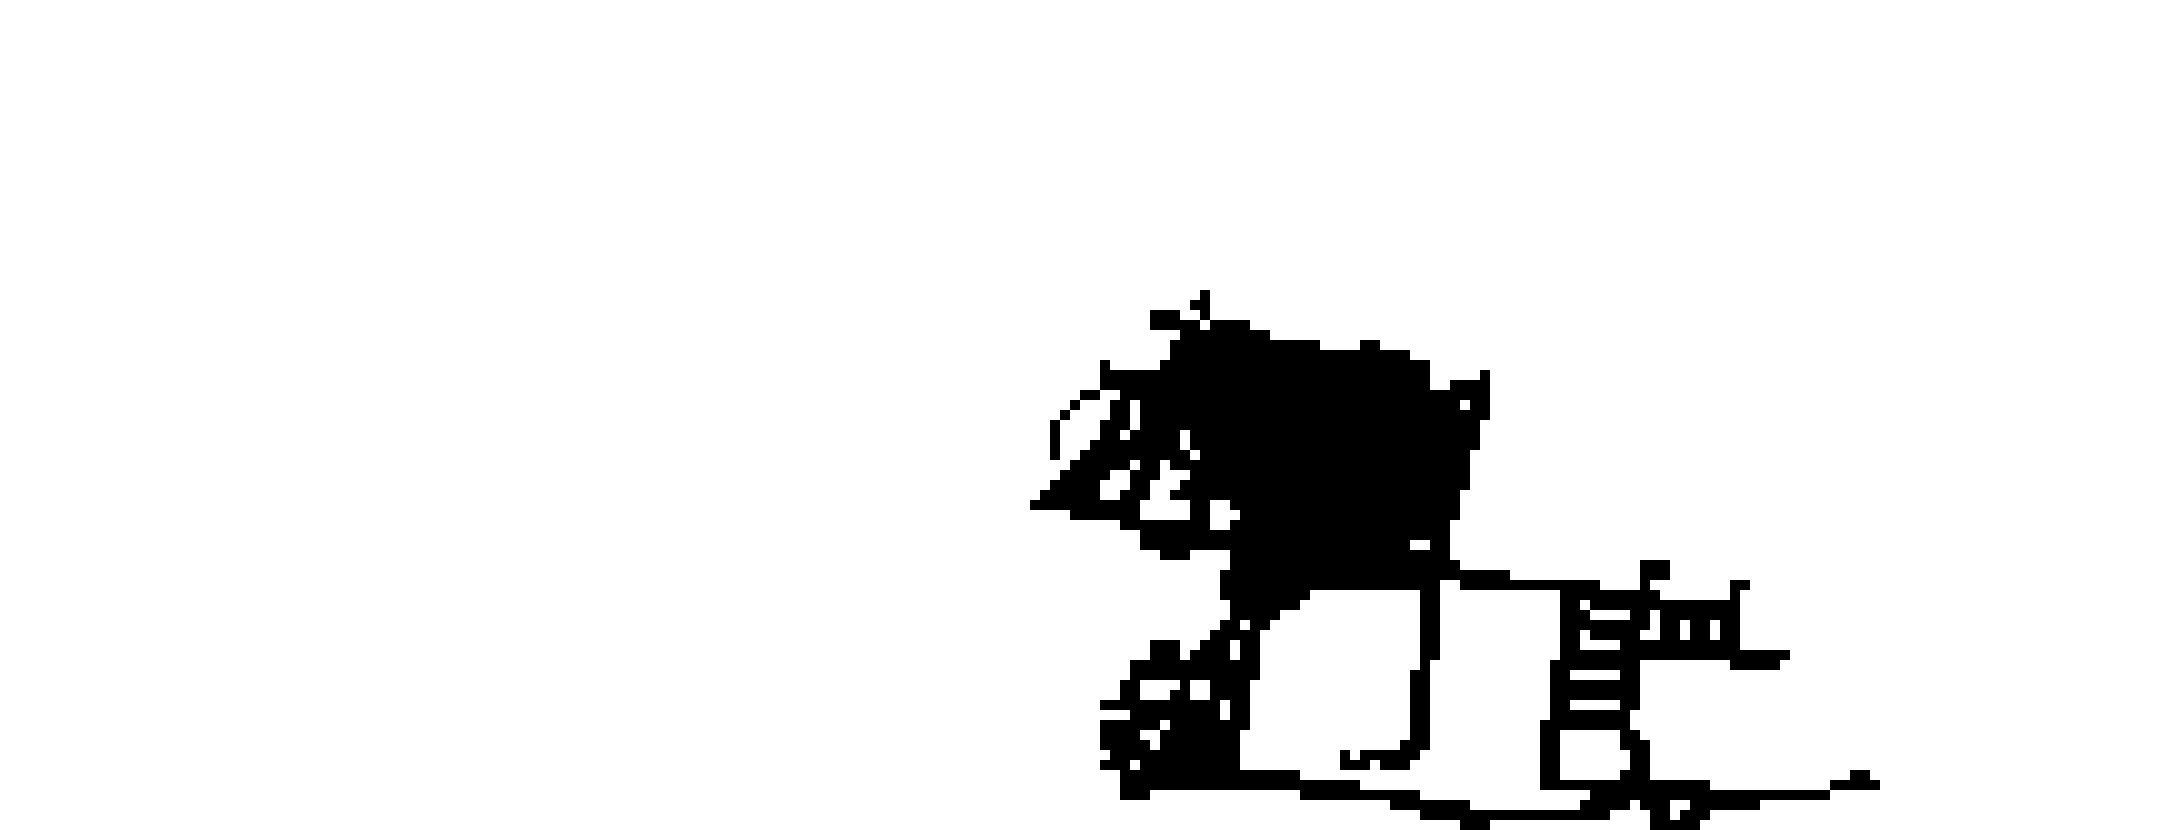
\includegraphics[width=1\linewidth]{Figures/Chapter4/generation-5-melusi}
  \caption*{Time step $t = 5$}
\end{subfigure}
\begin{subfigure}{.5\textwidth}
  \centering
  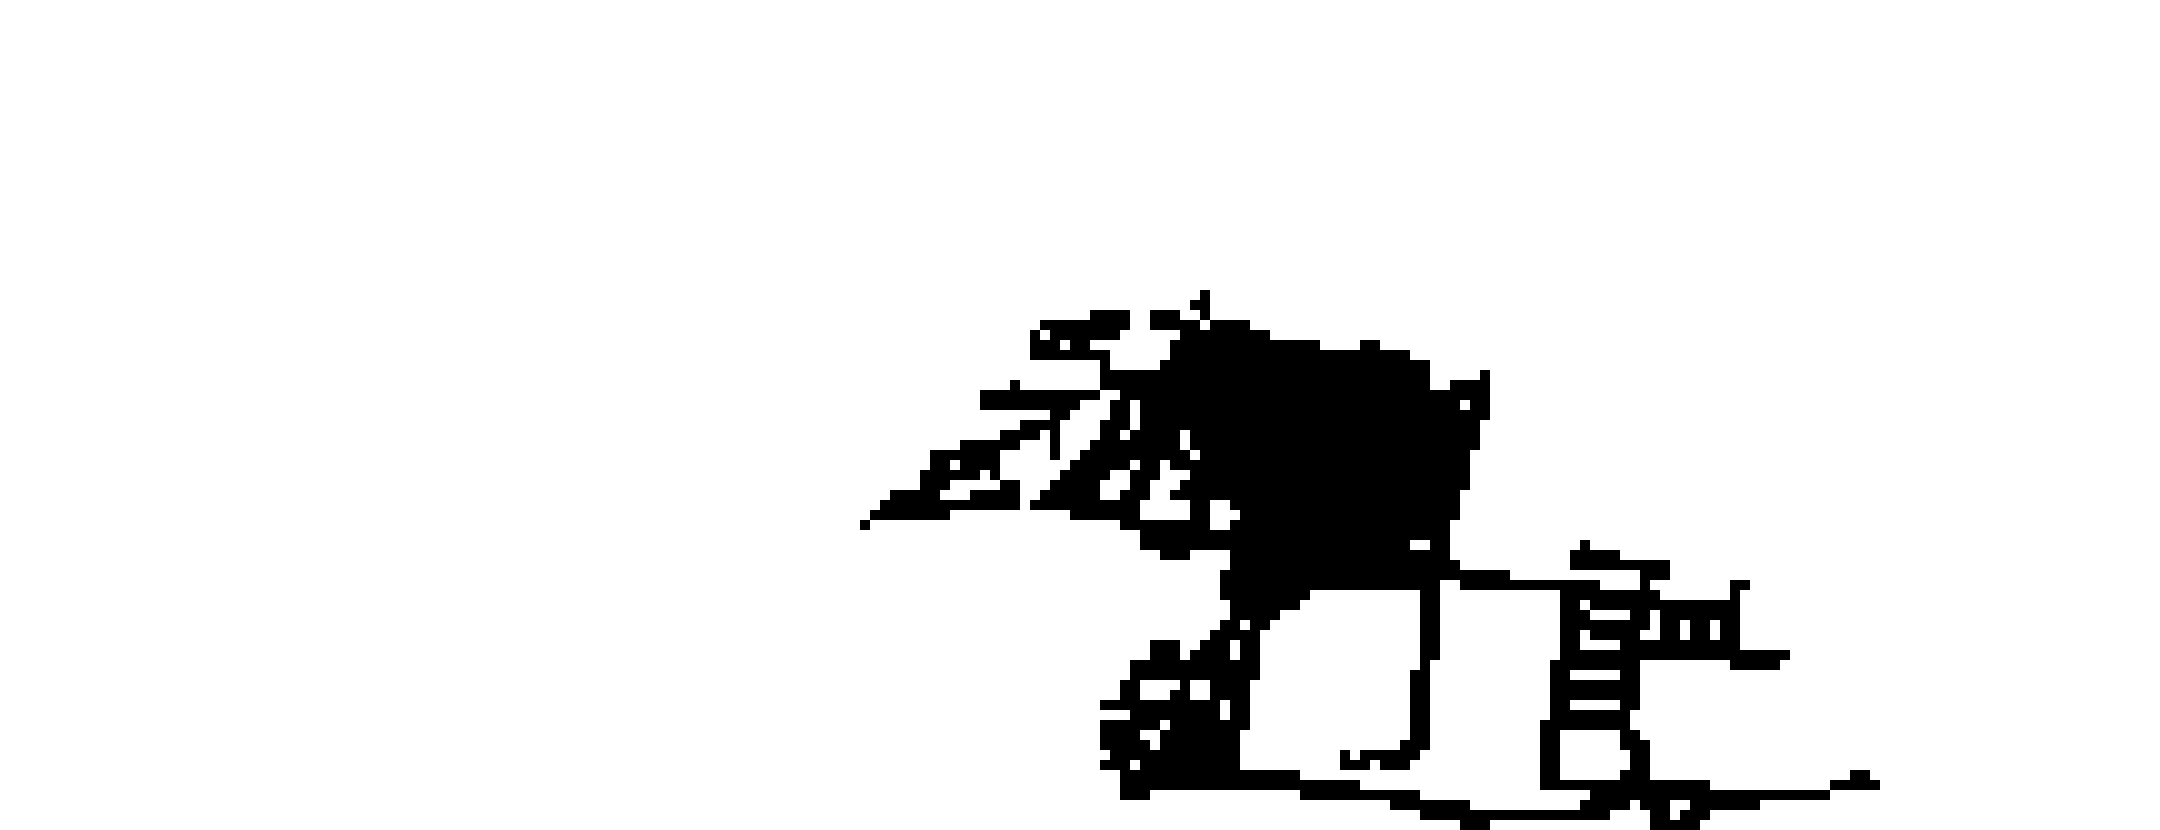
\includegraphics[width=1\linewidth]{Figures/Chapter4/generation-10-melusi}
  \caption*{Time step $t = 10$}
\end{subfigure}
\end{figure}

\begin{figure}[H]
\begin{subfigure}{.5\textwidth}
  \centering
  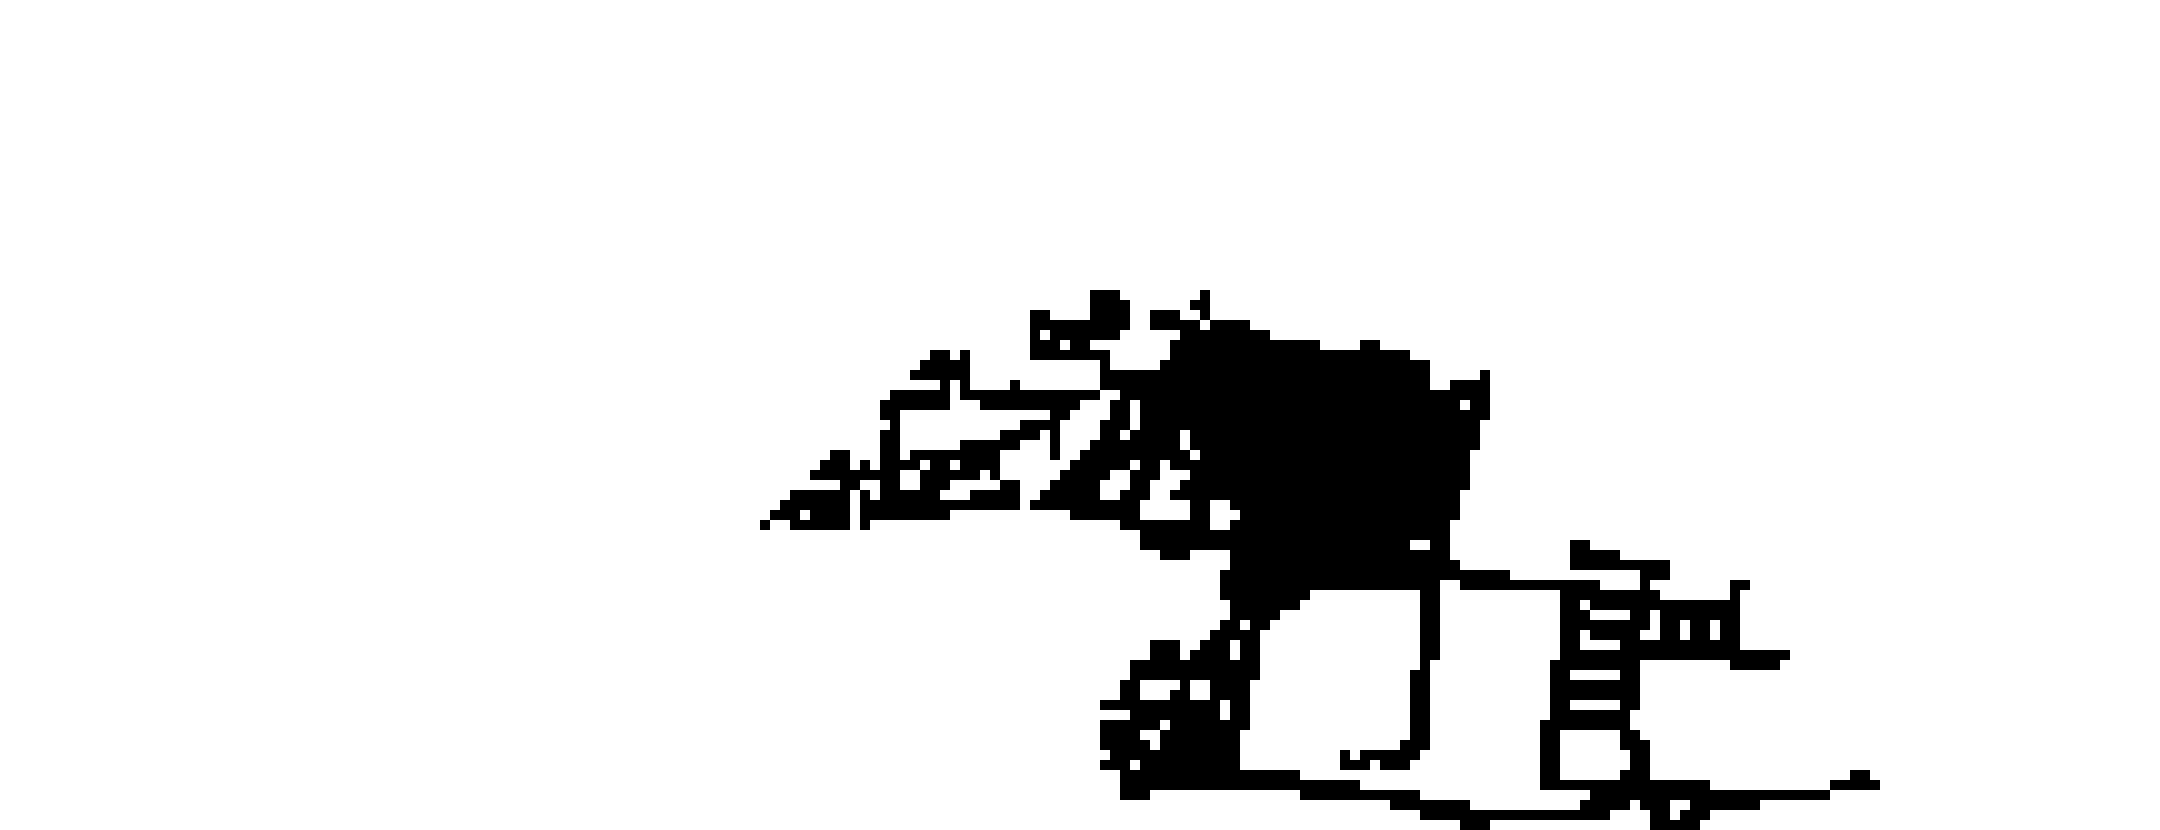
\includegraphics[width=1\linewidth]{Figures/Chapter4/generation-15-melusi}
  \caption*{Time step $t = 15$}
\end{subfigure}
\begin{subfigure}{.5\textwidth}
  \centering
  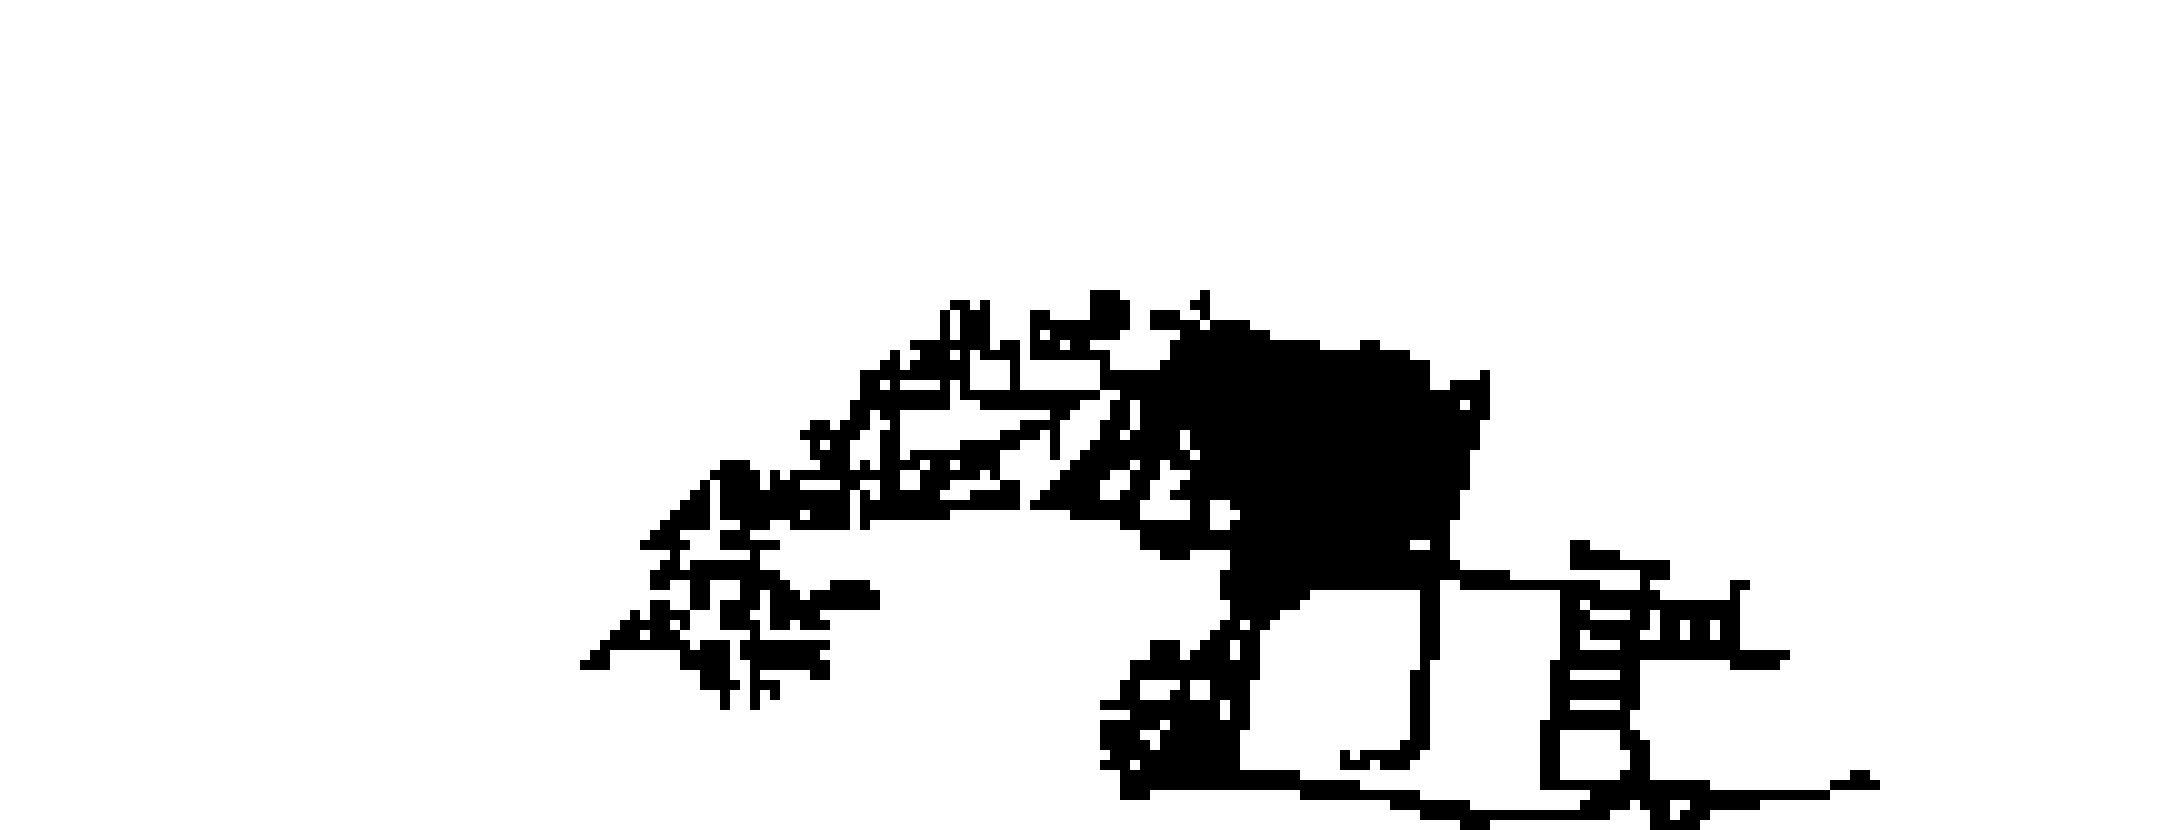
\includegraphics[width=1\linewidth]{Figures/Chapter4/generation-20-melusi}
  \caption*{Time step $t = 20$}
\end{subfigure}
\end{figure}

\begin{figure}[H]
\begin{subfigure}{.5\textwidth}
  \centering
  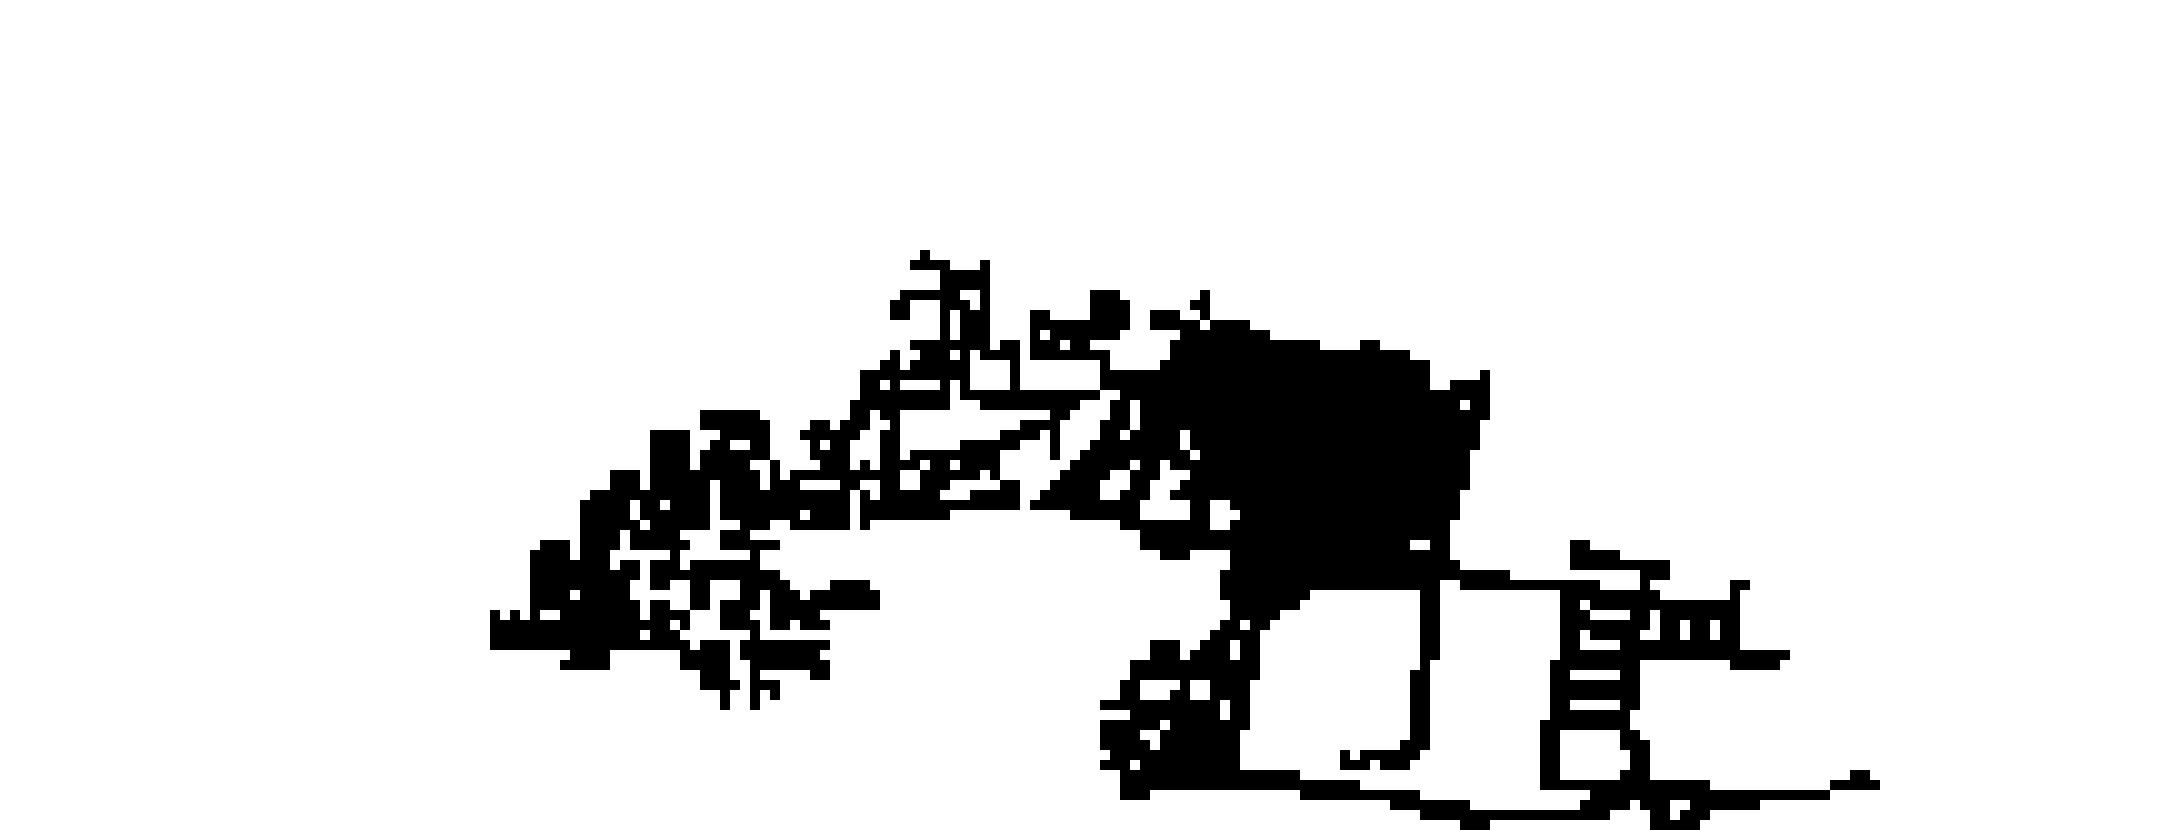
\includegraphics[width=1\linewidth]{Figures/Chapter4/generation-25-melusi}
  \caption*{Time step $t = 25$}
\end{subfigure}
\begin{subfigure}{.5\textwidth}
  \centering
  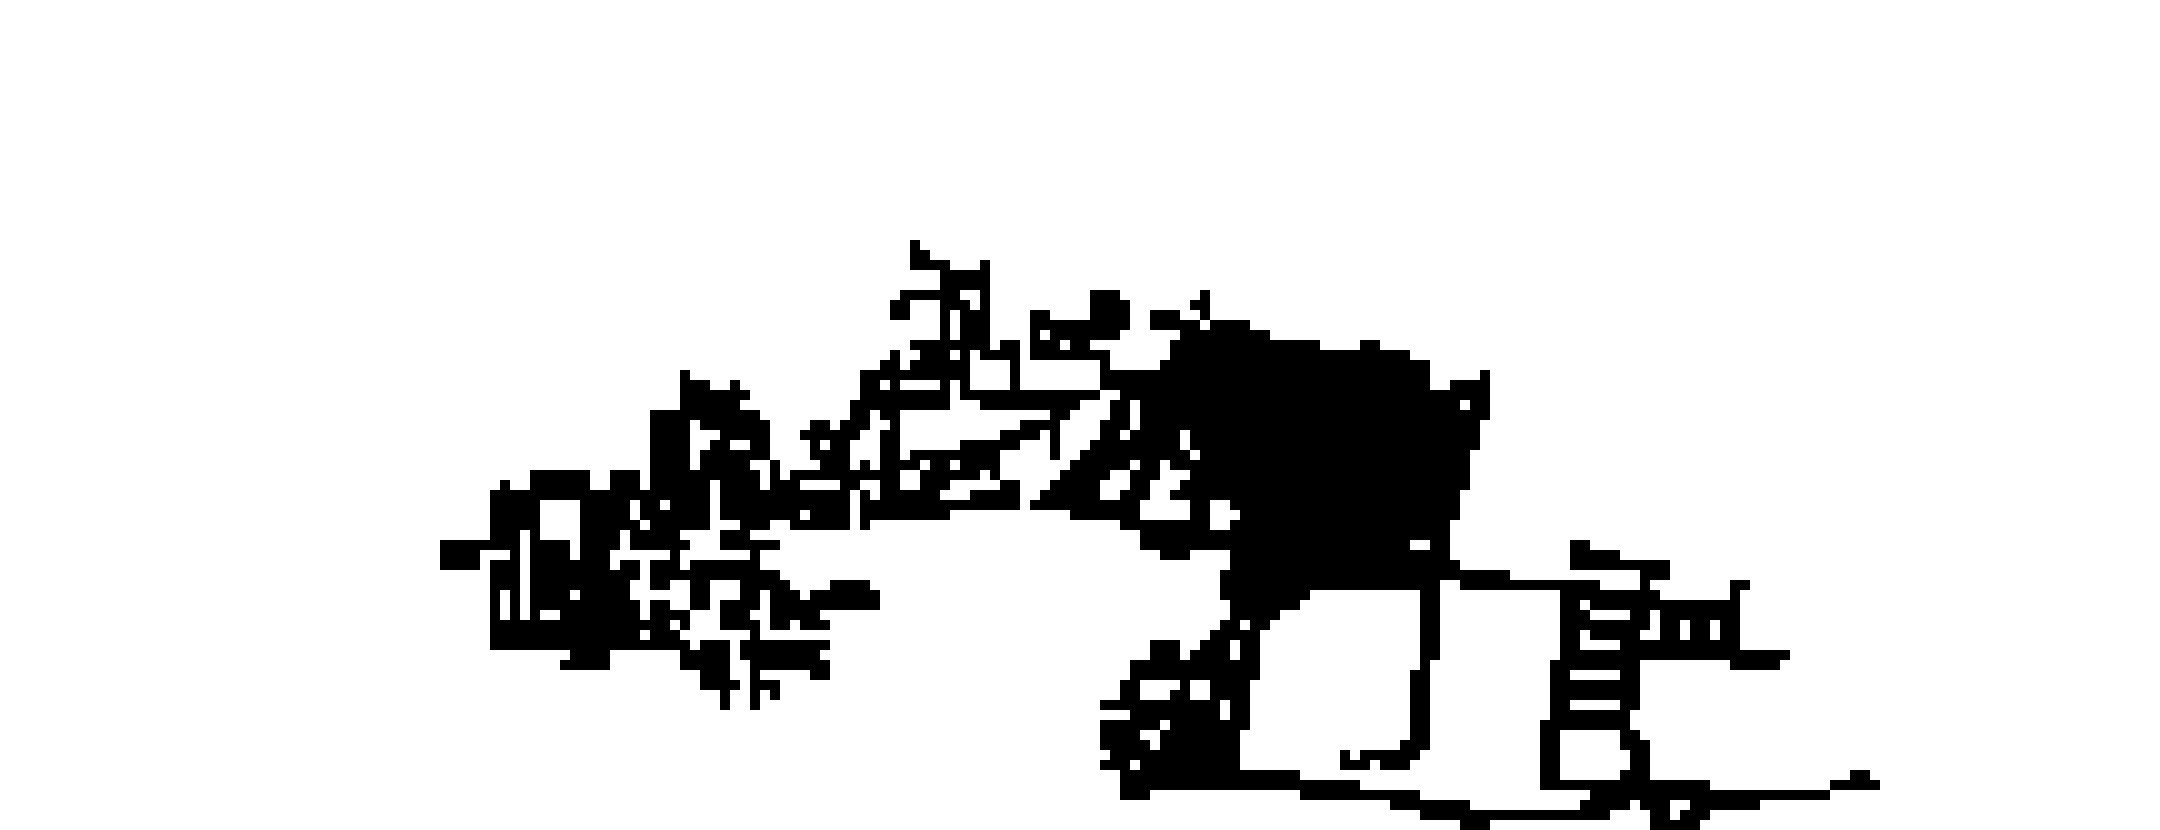
\includegraphics[width=1\linewidth]{Figures/Chapter4/generation-30-melusi}
  \caption*{Time step $t = 30$}
\end{subfigure}
\end{figure}

\begin{figure}[H]
\begin{subfigure}{.5\textwidth}
  \centering
  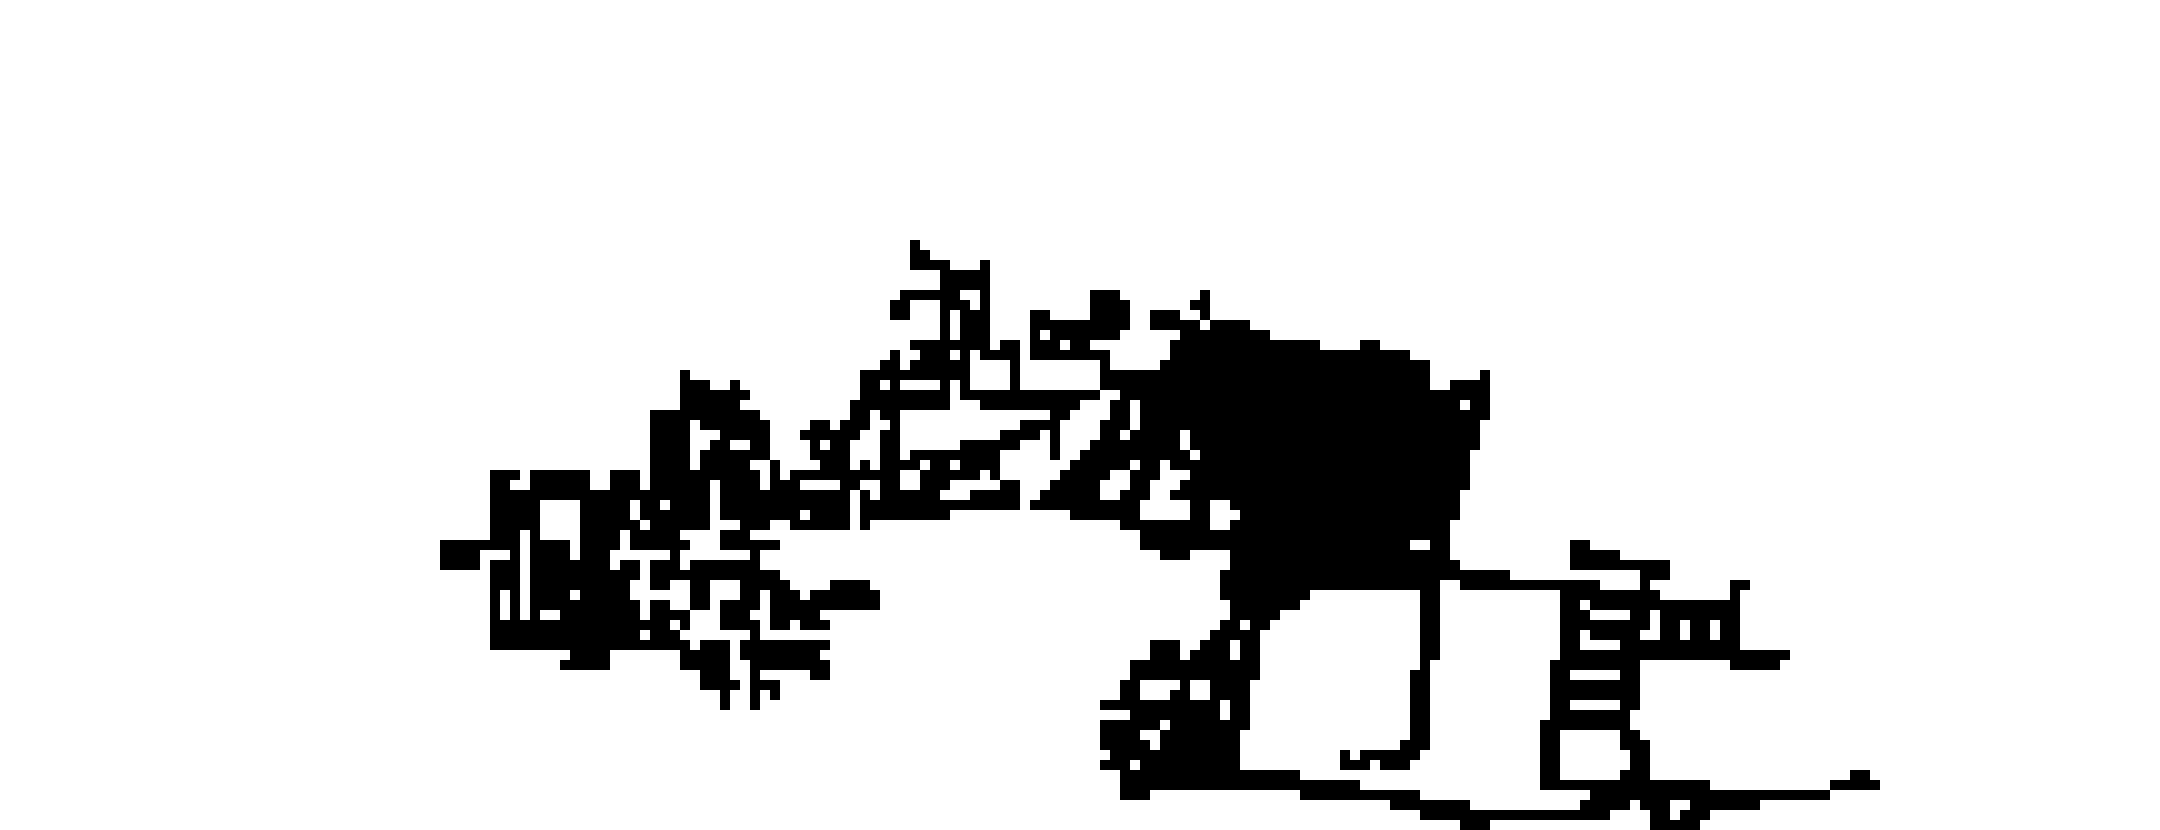
\includegraphics[width=1\linewidth]{Figures/Chapter4/generation-35-melusi}
  \caption*{Time step $t = 35$}
\end{subfigure}
\begin{subfigure}{.5\textwidth}
  \centering
  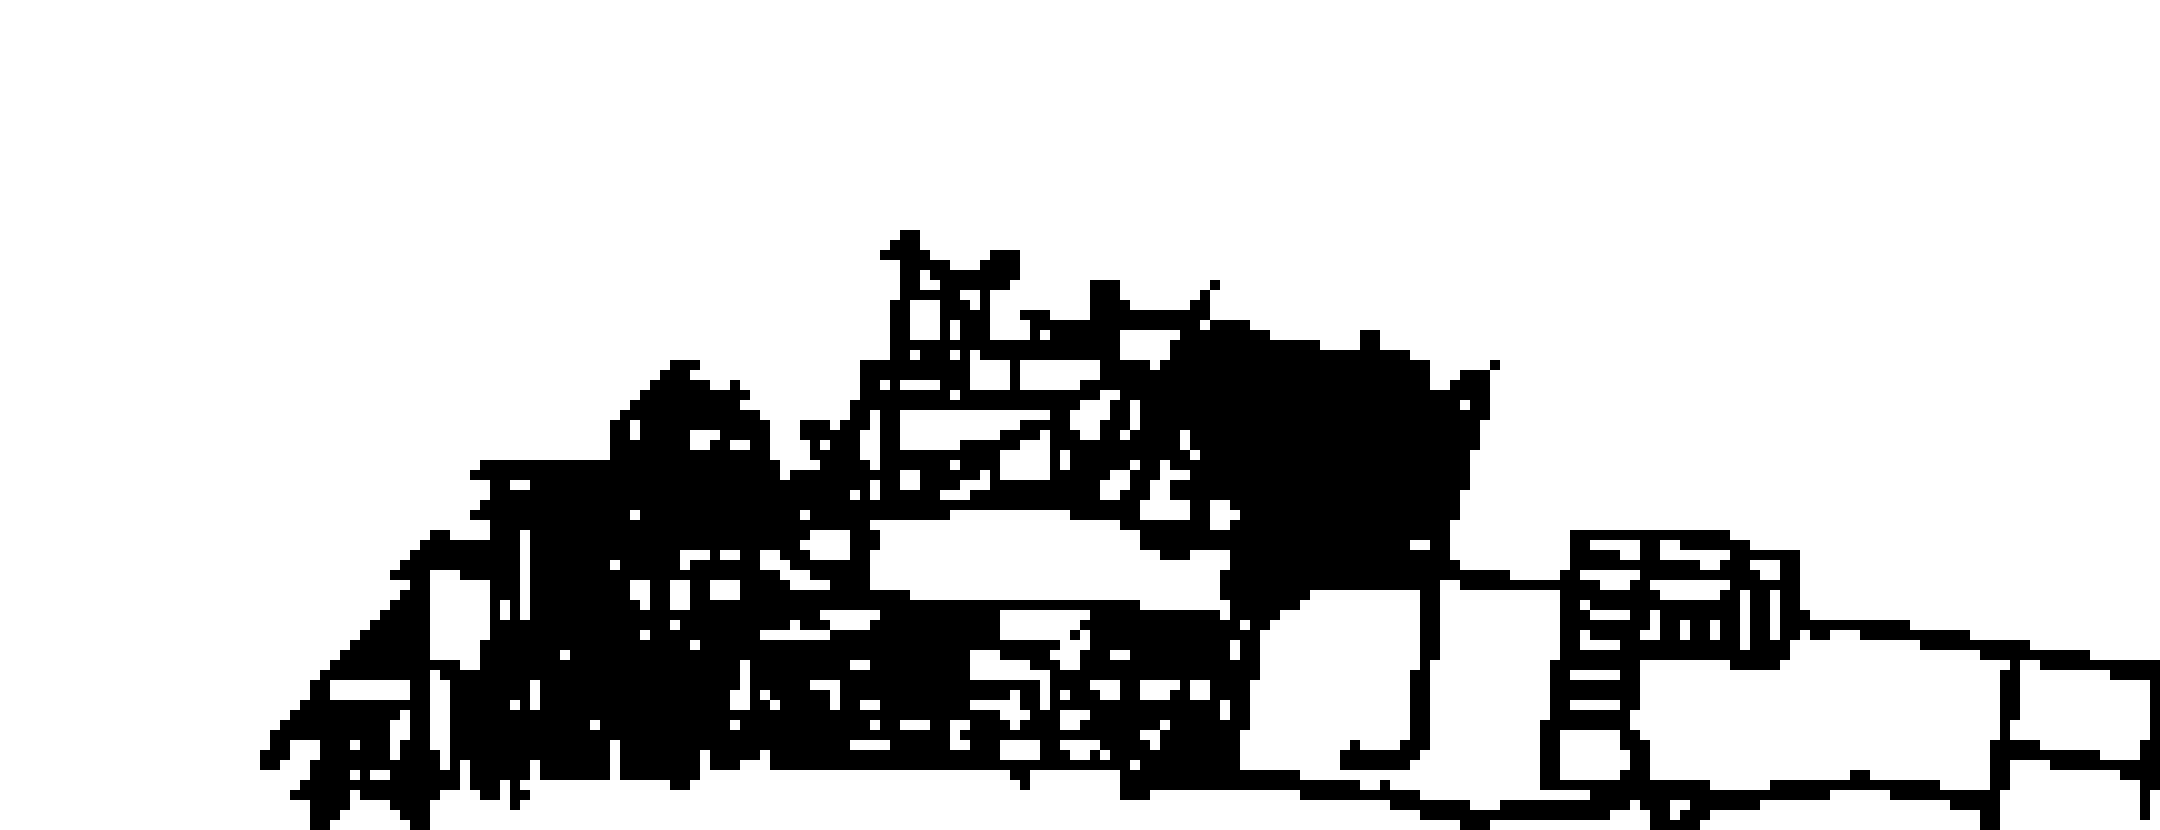
\includegraphics[width=1\linewidth]{Figures/Chapter4/generation-40-melusi}
  \caption*{Time step $t = 40$}
\end{subfigure}
\end{figure}

\begin{figure}[H]
\begin{subfigure}{.5\textwidth}
  \centering
  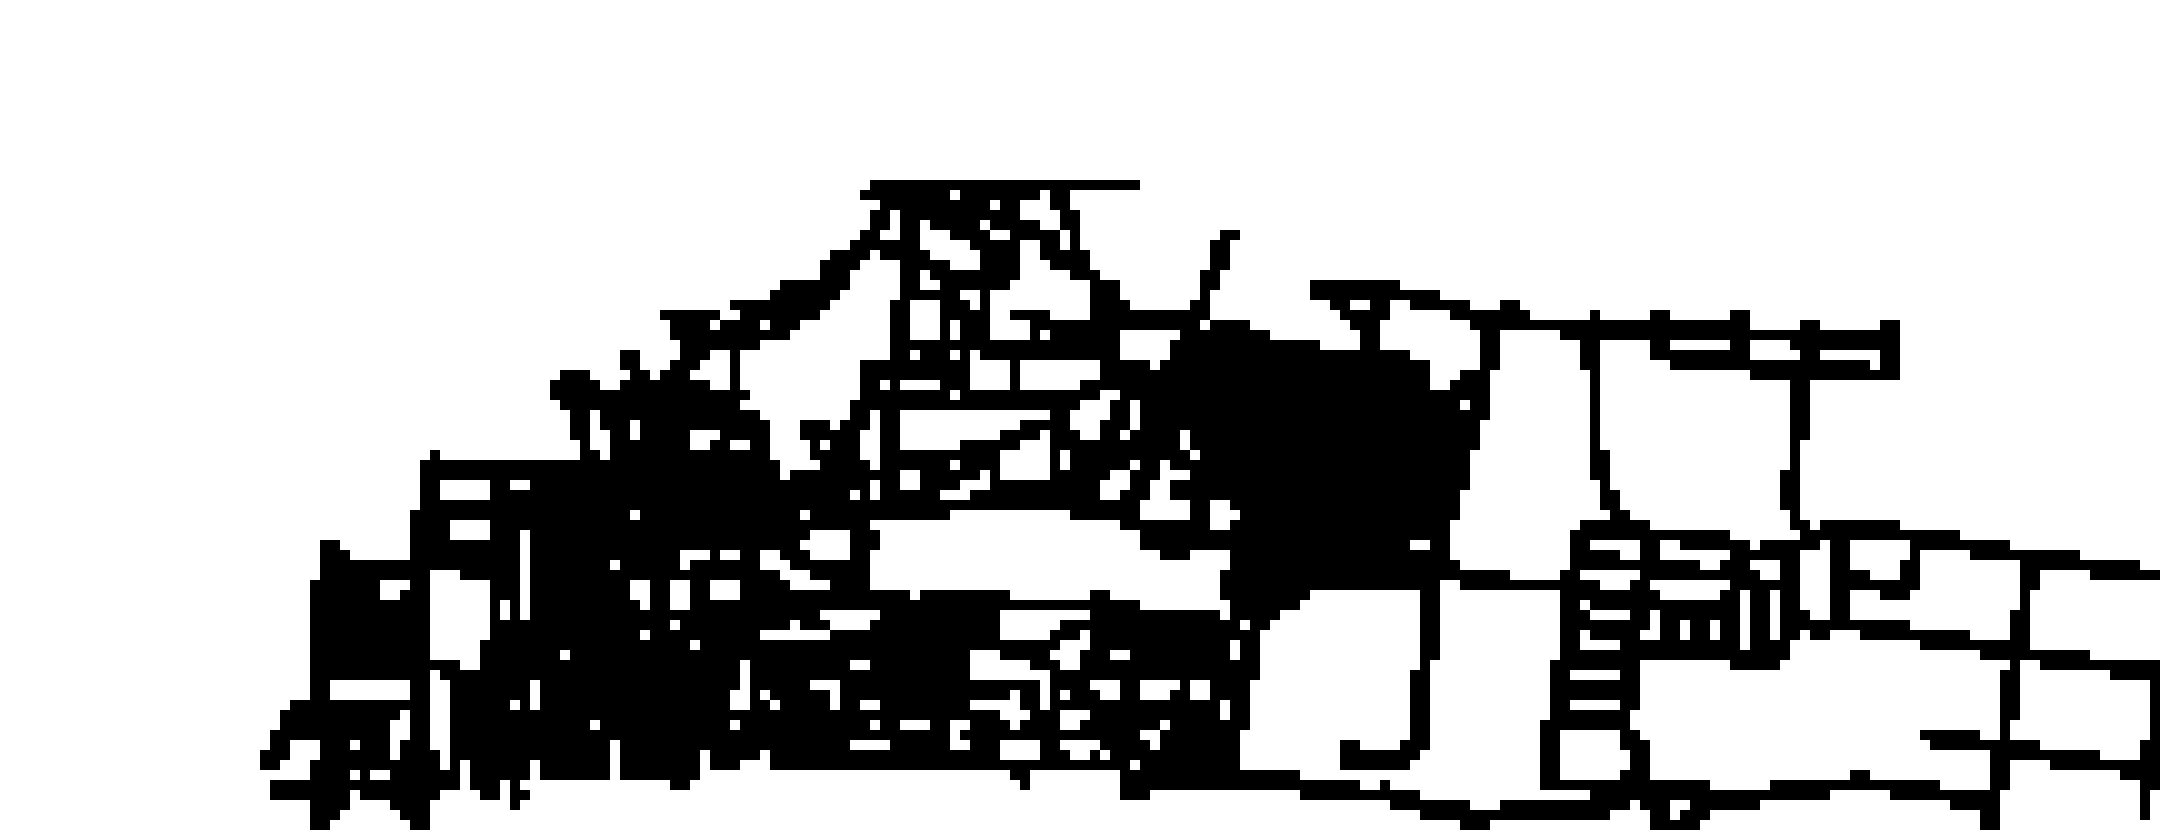
\includegraphics[width=1\linewidth]{Figures/Chapter4/generation-45-melusi}
  \caption{Time step $t = 45$}
\end{subfigure}
\begin{subfigure}{.5\textwidth}
  \centering
  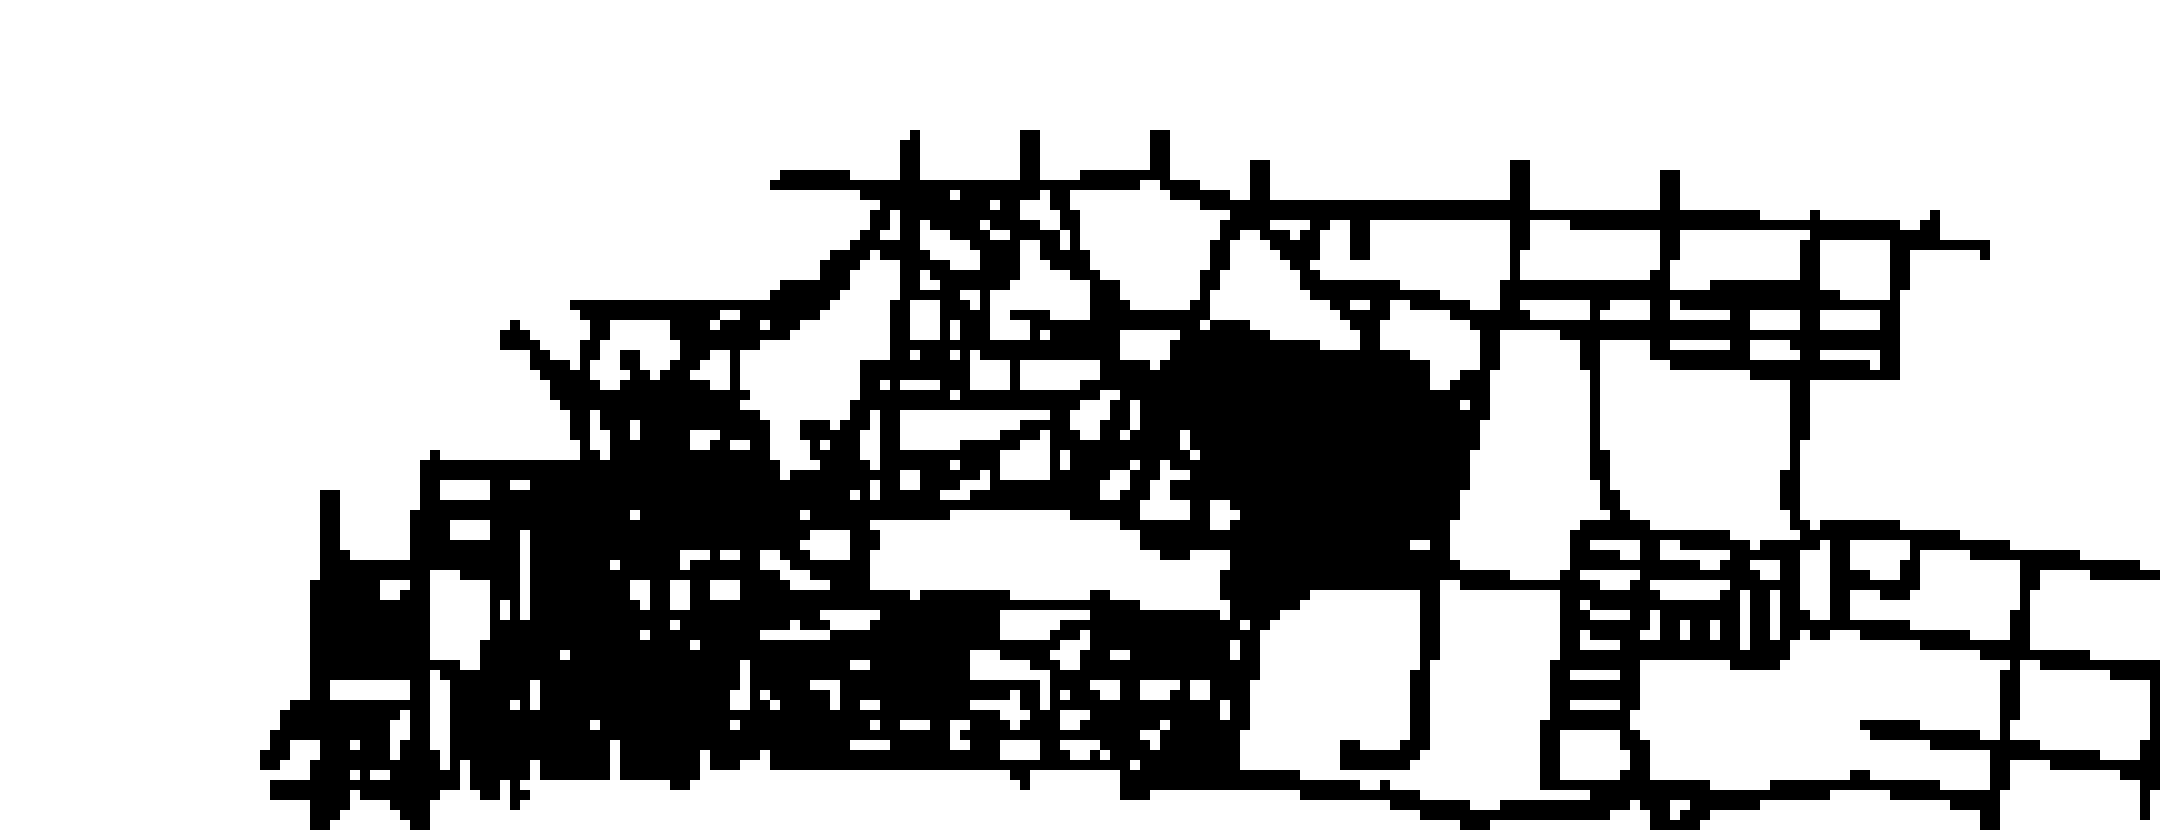
\includegraphics[width=1\linewidth]{Figures/Chapter4/generation-50-melusi}
  \caption{Time step $t = 50$}
\end{subfigure}
\caption{Simulated Growth of Building Based Land Usage for 50 time steps}
\label{fig:gen50}
\end{figure}
\begin{center}
Source: Own Creation (2021)
\end{center}
The second approach in the Visual comparisons metric was to create two images.
\begin{enumerate}
\item An image that overlays the Simulated Growth of the Building Based Land Usage on top of a General Reference Map.
\item An image that overlays the Actual or Existing Building Based Land Usage on top of a General Reference Map.
\end{enumerate}
The images for the above are seen in Figures \ref{fig:simmap} and \ref{fig:curmap} respectively. The validity of the CA model was then seen visually.
\\\\
Going back to the Kappa coefficient, a graph and a table was created to visualise the performance of the CA model over the 50 time steps. The former is seen in Figure \ref{fig:scores} and the later in Table \ref{table:kap2}.

The highest coefficient achieved was at the time step 45 with a value of \texttt{0.61775529641454560}. If this is compared to the Magnitude guidelines in Table \ref{table:kap} it falls under the "Substantial agreement" option. This is competent enough for the level of this research study. On the other hand, research cited in this paper had the Kappa coefficient range from 0.5 to 0.99. Therefore the results achieved in this study are admirable as well as sufficient.

Additionally, the research cited also was of a higher standard and sophisticated calibre. The culmination of this research study was achieved with just two variables, namely the Population density (Social Factor) and the Road networks (Infrastructure Factor).

However, on the downside the CA model did appear to drop accuracy in the last few time steps. This can be attributed to the following inferences made by the author:
\begin{itemize}
\item Although the original data of the Roads and Population Density was limited to just the \textit{Melusi} area, the limited area was a fixed bounding box. This box also encompassed roads that lead to other areas, and the Population Density of said areas. The approach to calculate the accuracy was discussed in Section \ref{sec:runmod}, therefore once the model decided to venture out of the \textit{Melusi} area in time step 45, the accuracy dropped.
\item The rules for time steps 40 and above became a bit too unstable or possibly chaotic in nature.
\item From reviewing the relevant literature it has been stated that Cellular Automata given certain initial states can branch out over the balance of Order into Chaos.
\end{itemize}
\begin{figure}[H]
\centering
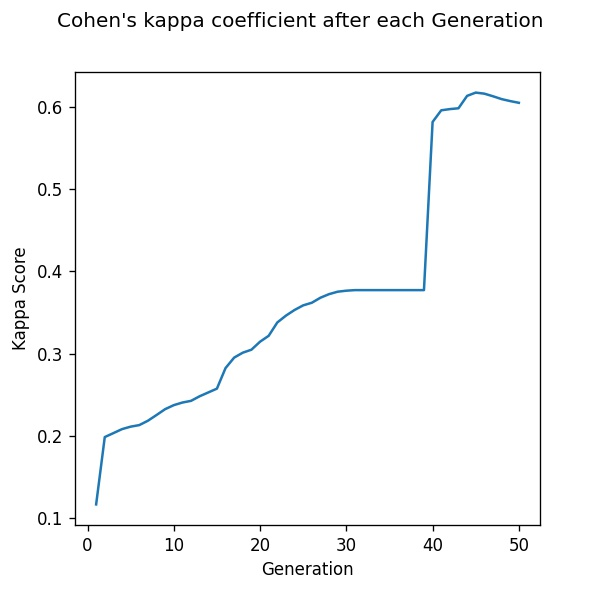
\includegraphics[scale=0.7]{Figures/Chapter4/scoresFigure}
\caption{Kappa coefficient for each Time step simulated}
\label{fig:scores}
\end{figure}

\begin{figure}[H]
\centering
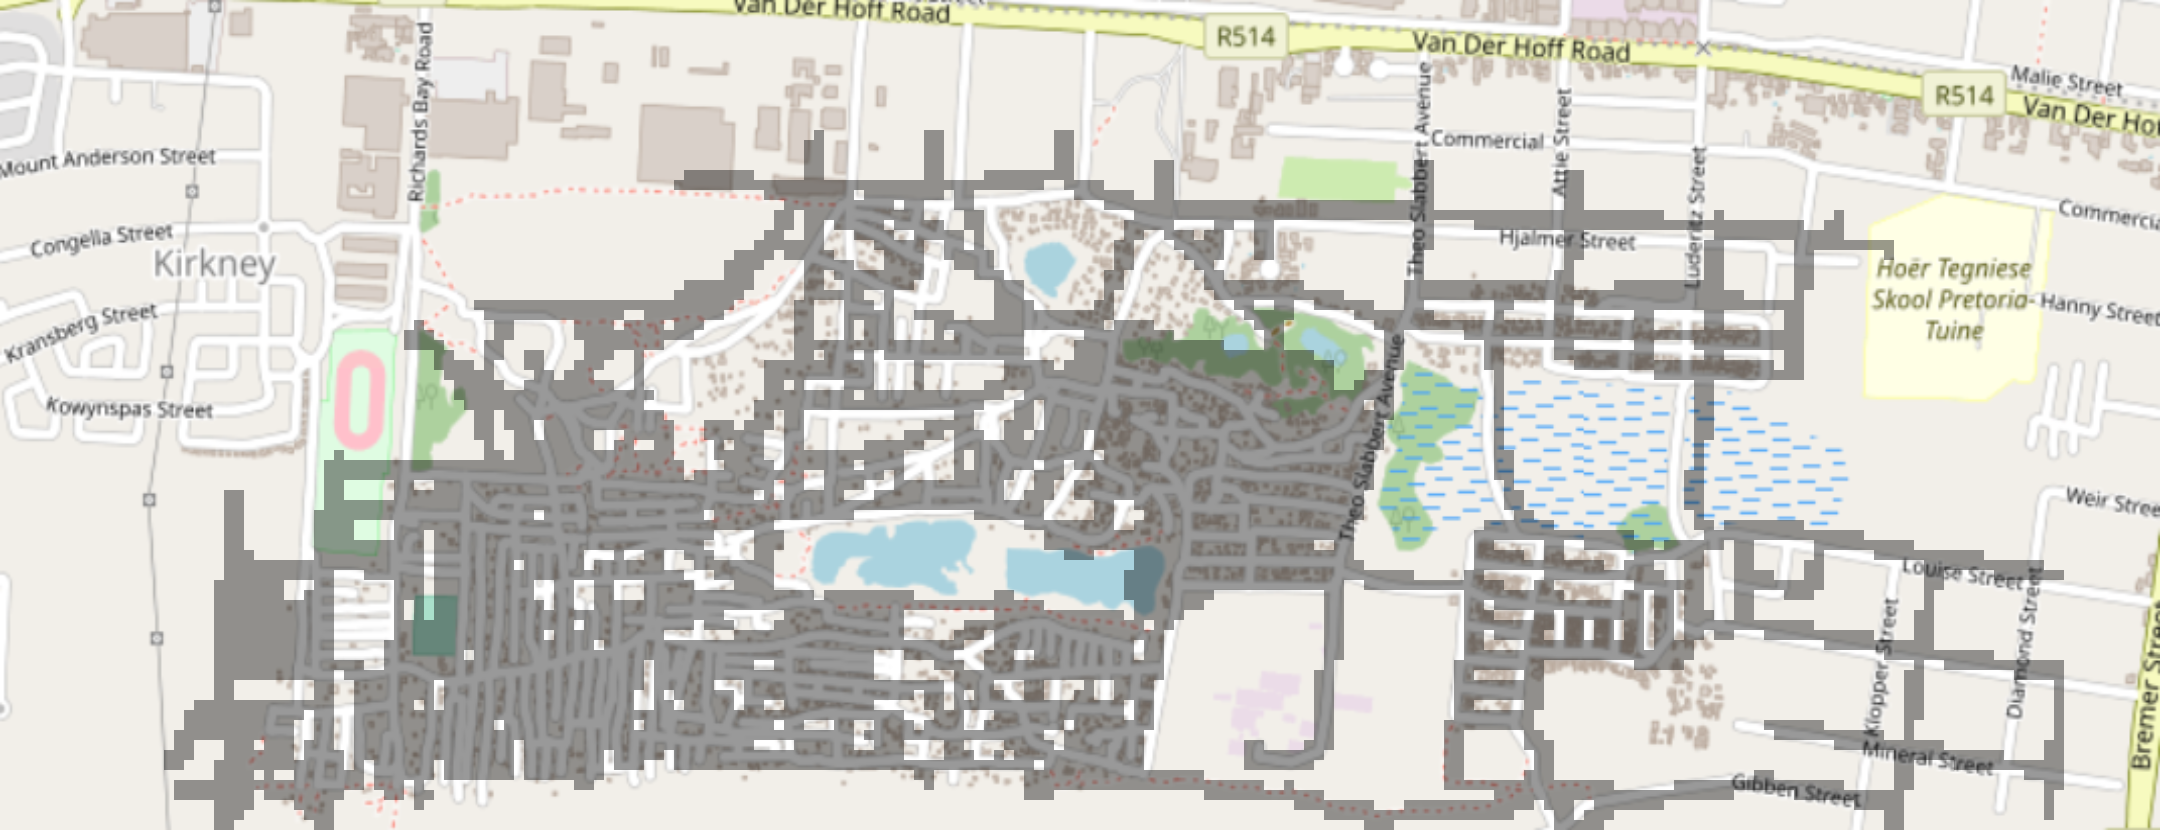
\includegraphics[scale=0.3,angle=90]{Figures/Chapter4/Simulated}
\caption{Simulated Growth of Building Based Land Usage on a Map}
\label{fig:simmap}
\end{figure}

\begin{figure}[H]
\centering
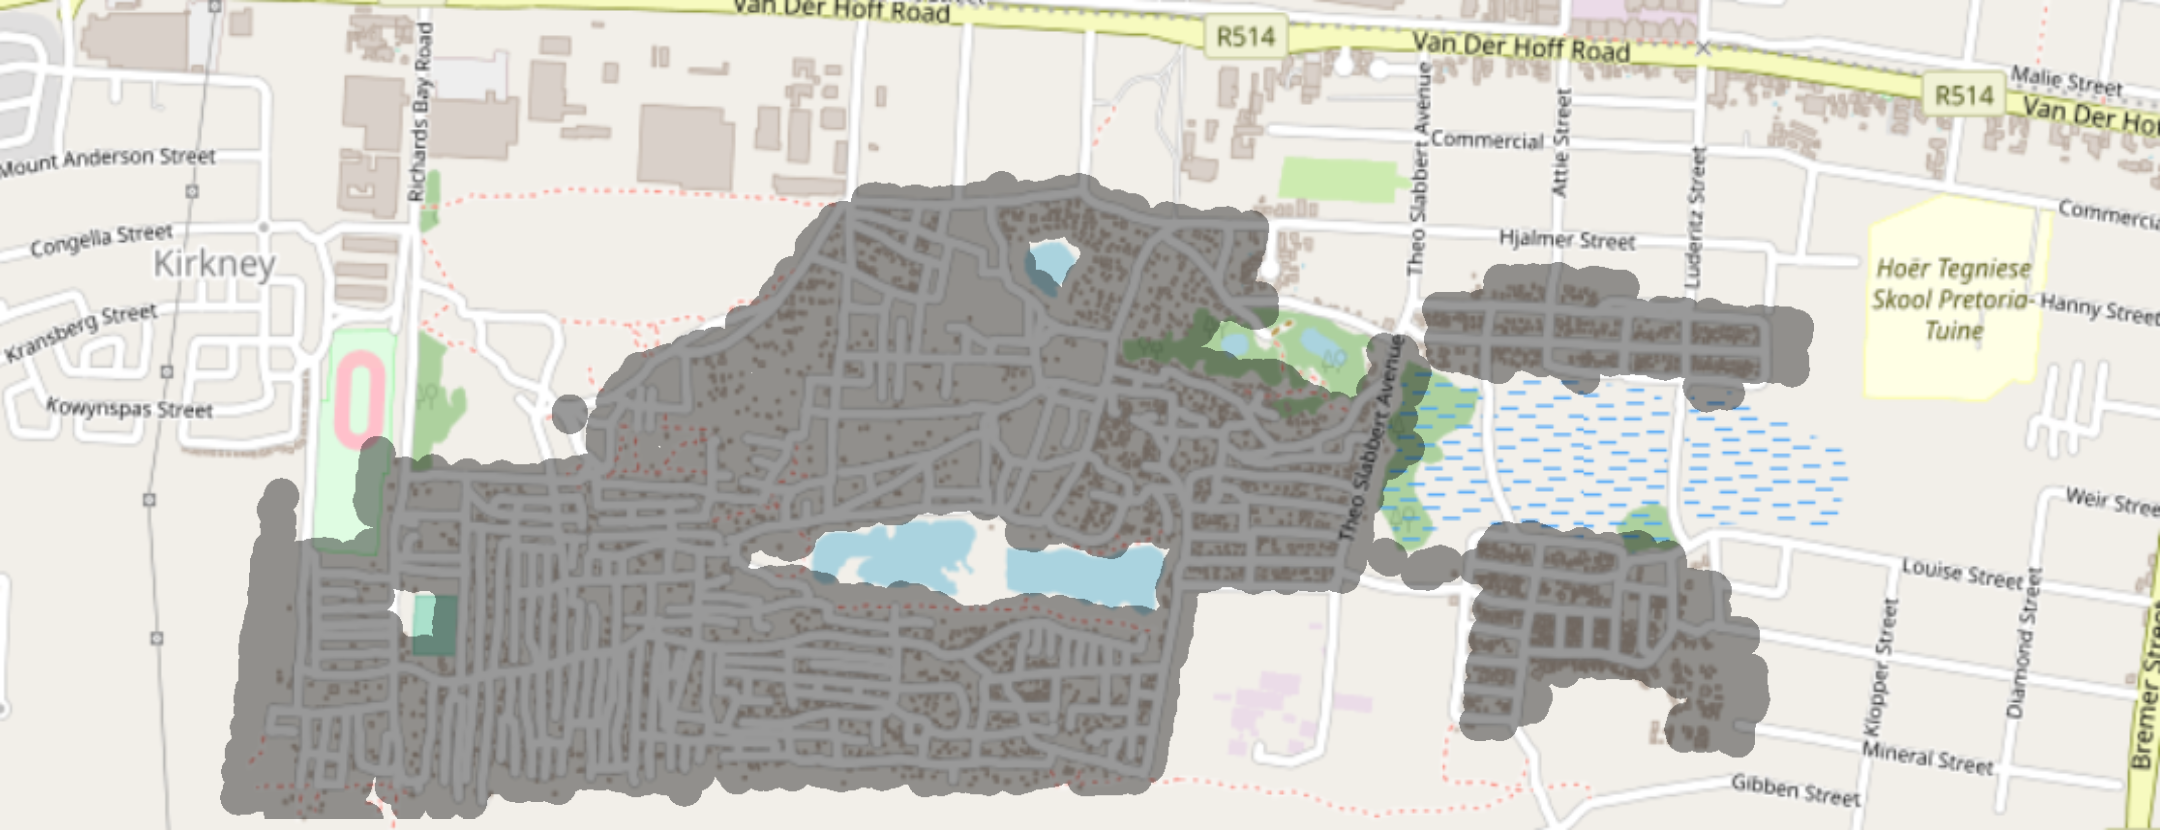
\includegraphics[scale=0.3,angle=90]{Figures/Chapter4/Actual}
\caption{Existing Building Based Land Usage on a Map}
\label{fig:curmap}
\end{figure}



\begin{table}[H]
\setlength{\tabcolsep}{12pt}
\renewcommand{\arraystretch}{1.1}
    \caption{Accuracy results for each time step}
    \label{table:kap2}
    \begin{minipage}{.5\linewidth}
      %\caption{}
            \begin{tabular}{@{}cl@{}}
            \toprule
            Time step & $\kappa$ coefficient \\ \midrule
            1 &  0.11625181498059378 \\
2 &  0.19824922121107136 \\
3 &  0.20306283544626080 \\
4 &  0.20793481429046645 \\
5 &  0.21093437785824343 \\
6 &  0.21283046681369622 \\
7 &  0.21812986043325577 \\
8 &  0.22511088417746883 \\
9 &  0.23225494066337948 \\
10 & 0.23712807908806854 \\
11 & 0.24030784142599682 \\
12 & 0.24236259441785502 \\
13 & 0.24795555301338124 \\
14 & 0.25260419032659376 \\
15 & 0.25724181362747820 \\
16 & 0.28227924369204370 \\
17 & 0.29504157655474317 \\
18 & 0.30102906854032363 \\
19 & 0.30464884852311600 \\
20 & 0.31438848428890310 \\
21 & 0.32157142237699610 \\
22 & 0.33780443805206917 \\
23 & 0.34613948926327110 \\
24 & 0.35302831352863406 \\
25 & 0.35866215860009740 \\ \bottomrule
        \end{tabular}
    \end{minipage}%
    \begin{minipage}{.5\linewidth}
        %\caption{}
        \begin{tabular}{@{}cl@{}}
          \toprule
          Time step & $\kappa$ coefficient \\ \midrule
          26 & 0.36182388889416850 \\
          27 & 0.36795669505675166 \\ 
          28 & 0.37232518280926630 \\
          29 & 0.37529002091648256 \\
          30 & 0.37650949057057026 \\
          31 & 0.37720597829276714 \\
          32 & 0.37720597829276714 \\
          33 & 0.37720597829276714 \\
          34 & 0.37720597829276714 \\
          35 & 0.37720597829276714 \\
          36 & 0.37720597829276714 \\
          37 & 0.37720597829276714 \\
          38 & 0.37720597829276714 \\
          39 & 0.37720597829276714 \\
          40 & 0.58197245681417580 \\
          41 & 0.59617325191136350 \\
          42 & 0.59765374964576660 \\
          43 & 0.59865025952753870 \\
          44 & 0.61375538510117190 \\
          \textcolor{Green}{\textbf{45}} & \textcolor{Green}{\textbf{0.61775529641454560}} \\
          46 & 0.61644571800015240 \\
          47 & 0.61328585200053230 \\
          48 & 0.60982488474318350 \\
          49 & 0.60740162003478520 \\
          50 & 0.60532388693353810 \\ \bottomrule
      \end{tabular}
      %\vspace*{0.8in}
    \end{minipage}
\end{table}